% !TEX root = ejemplo.tex

\chapter{Fuentes}
Para las fuentes del documento he escogido los paquetes \texttt{fontspec} y
\texttt{unicode-math} en el caso de compilar con Lua\LaTeX. Si la
compilación es con pdf\LaTeX{} se usarán los paquetes \texttt{inputenc} y
\texttt{fontenc}.

La ventaja de \texttt{fontspec} y \texttt{unicode-math} es que posible
cambiar fuentes de manera fácil en partes del documento, pero deberá ser
compilado con Xe\LaTeX{} o con Lua\LaTeX, el último siendo el método
recomendado. Con esto se podrán usar caracteres unicode en cualquier parte
de texto, por ejemplo en una ecuación centrada (para que aparezcan las
ecuaciones compila con Lua\LaTeX.)
\ifluatex%
\[
  ∀ε>0∃δ>0(|x-y|<δ ⇒ |f(x)-f(y)|<ε)
\]
\else
\ifpdftex%
\begin{center}
\textcolor{red}{La compilación con pdf\LaTeX{} no permite mostrar este
ejemplo.}
\end{center}
\fi
\fi
o en una línea de texto%
\ifluatex%
\(∀ε>0∃δ>0(|x-y|<δ ⇒ |f(x)-f(y)|<ε)\).
\else
\ifpdftex%
\textcolor{red}{La compilación con pdf\LaTeX{} no permite mostrar este
ejemplo.}
\fi
\fi
Las letras griegas, por ejemplo, no necesitan estar en modo matemático para
funcionar
\ifluatex%
αβγδφψ
\else
\ifpdftex%
\textcolor{red}{La compilación con pdf\LaTeX{} no permite mostrar este
ejemplo.}
\fi
\fi
(ver código fuente ignorando los condicionales para cada tipo de
compilación).

La fuente que fue escogida para este texto es \textit{Stix Two}. Esta fuente
tiene como objetivo servir como un estándar para la preparación, publicación
e impresión de textos científicos. Es impulsada y usada por la \textit{AMS}
(matemáticas), \textit{ACS} (química), \textit{AIP} y \textit{APS} (física),
\textit{IEEE} (ingeniería) y Elsevier. Por lo tanto, tiene un conjunto de
símbolos sumamente extenso.

Para nuestros ejemplos, con Lua\LaTeX, se cambiara el tipo de fuente sans
por GFS Neohellenic. No es recomendable usar muchos tipos de fuente en un
documento, pero como esto es un ejemplo haremos dicho cambio. Como distintas
fuentes tienen distintos tamaños, al combinar dos de ellas es muy posible
crear una inconsistencia en los tamaños. Para evitar esto use la opción de
\texttt{fontspec} (ver preámbulo) \texttt{Scale=MatchUppercase}. Este
paquete puede hacer muchas modificaciones a los atributos de una fuente y no
veremos más de esos atributos. En el preámbulo está la definición de un
ambiente donde la fuente se cambia:
\ifluatex%
\begin{sans}%
\label{textosans}
  \lipsum[1][1-3]
  \[
    \prod_{i\in I}A_i\ne\emptyset
  \]
\end{sans}
Como el objetivo fue cambiar la fuente sans el cambio también se hará al usar
\verb|\textsf{...}| y \verb|{\sffamily ...}| como podemos ver a continuación
\textsf{cambio de fuente
\mathversion{sansmath}\(\forall\varepsilon>0\exists\delta>0(\ldots)\)}. Como
puede verse en el ejemplo lo que hace cambiar la fuente matemática es el
comando \verb|\mathversion{sansmath}| de \texttt{unicode-math}.
\else
\ifpdftex%
\begin{center}
\textcolor{red}{La compilación con pdf\LaTeX{} no permite mostrar este
ejemplo.}
\end{center}
\fi
\fi

Un ejemplo de dónde se hizo este tipo de cambios es en las Lecturas de Física
de Feynman. En este texto las figuras llevan un tipo de fuente diferente a la
del cuerpo.
\ifluatex%
\begin{figure}[h]
\mathversion{sansmath}
\centering
\begin{minipage}{0.4\linewidth}
\centering
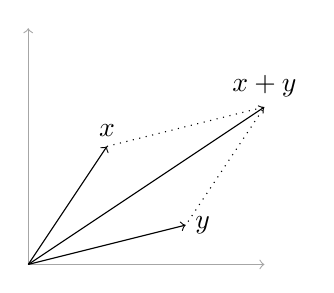
\begin{tikzpicture}
  \draw[gray!70,->] (0,0) -- (3,0);
  \draw[gray!70,->] (0,0) -- (0,3);
  \draw[->] (0,0) -- (1,1.5) node[above] {\(x\)};
  \draw[->] (0,0) -- (2,0.5) node[right] {\(y\)};
  \draw[->] (0,0) -- (3,2) node[above] {\(x+y\)};
  \draw[dotted] (1,1.5) -- (3,2) -- (2,0.5);
\end{tikzpicture}

  \captionnamefont{\sffamily}
  \subcaption{\sffamily Suma de vectores}
  \label{fig:vect1}
\end{minipage}
\hfill
\begin{minipage}{0.4\linewidth}
\centering
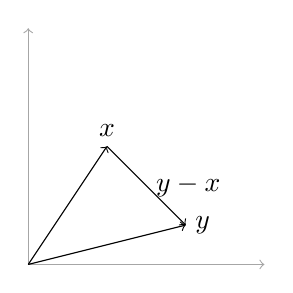
\begin{tikzpicture}
  \draw[gray!70,->] (0,0) -- (3,0);
  \draw[gray!70,->] (0,0) -- (0,3);
  \draw[->] (0,0) -- (1,1.5) node[above] {\(x\)};
  \draw[->] (0,0) -- (2,0.5) node[right] {\(y\)};
  \draw[->] (1,1.5) -- node[right] {\(y-x\)} (2,0.5);
\end{tikzpicture}

  \captionnamefont{\sffamily}
  \subcaption{\sffamily Resta de vectores}
  \label{fig:vect2}
\end{minipage}
  \captionnamefont{\sffamily}
  \caption{\sffamily Operaciones con vectores}
  \label{fig:vect}
\end{figure}
\else
\ifpdftex%
\begin{center}
\textcolor{red}{La compilación con pdf\LaTeX{} no permite mostrar este
ejemplo.}
\end{center}
\fi
\fi

Como no está pensado para que así sea la salida de todas las figuras no se
hizo la definición en el preámbulo. Para dicho cambio se debe escribir
\verb|\captionnamefont{\sffamily}| para cambiar el tipo de fuente de la
palabra \enquote{Figura} y su número. Para cambiar el delimitador, que en este caso
son dos puntos se usa \verb|\captiondelim{: }|. Para cambiar el tipo de
fuente del título de las figuras se usa \verb|\captiontitlefont{\sffamily}|.
Con esto es fácil hacer una configuración de la salida de los títulos de
figuras y tablas, también se podría cambiar el tamaño de la fuente o poner
alguna palabra en específico.

Otra ventaja del manejo de fuentes de Xe\LaTeX{} y Lua\LaTeX{} es que las
fuentes instaladas en nuestro sistema estarán disponibles para su uso en
documentos de \LaTeX{}. Por ejemplo si quisiéramos que nuestro documento
estuviera escrito en Arial simplemente hay que escribir
\begin{flushleft}
  \verb|\setmainfont{Arial}|
\end{flushleft}
contrario a la forma en la que hace pdf\LaTeX{} donde habría que usar el
código de la fuente y en muchos casos es difícil encontrar dicho código.
Además que las fuentes disponibles de esa forma son relativamente pocas.
Para dar una idea de la disponibilidad de fuentes con Xe\LaTeX{} y
Lua\LaTeX{} basta ver las fuentes disponibles en overleaf \url{https://www.overleaf.com/latex/examples/fontspec-all-the-fonts/hjrpnxhrrtxc}.
Seguramente en tu sistema habrá un conjunto de fuentes disponibles grande.

\ifluatex%
Un comentario acerca de \texttt{unicode-math} es que permite usar una
fuente específica para cada alfabeto. El ejemplo en este texto es cambiar la
fuente script, que tanto en \textit{Stix two} como muchas otras fuentes es
igual a la caligráfica. Con \texttt{unicode-math} es suficiente cargar una
fuente con el alfabeto que nos guste, sólo para el rango que la queremos.
Aún cuando en un principio no es necesario tener tantos alfabetos matemáticos
diferentes, en teoría de categorías he visto una notación que aunque no es
estándar (creo que aún no hay ningún estándar) parece dar coherencia. Las
categorías pequeñas y localmente pequeñas se denotan con letras en negritas
\(\mbfA \), \(\symbf{Con}\),\ldots categorías más grandes se denotan con
letras caligráficas \(\mathcal{X}\), \(\symcal{Y}\), etc. y categorías
especiales como topos se denotan con letras script como \(\symscr{E}\).

En el código se puede notar que se han usado diferentes sintaxis para los
alfabetos, que \texttt{unicode-math} se encargará de mapear al símbolo
correcto. Por ejemplo, las formas de obtener la letra \enquote{A} en negritas es
como símbolo definido por un alfabeto \verb|\mbfA|, como comando de
\texttt{unicode-math} (es la forma recomendada) \verb|\symbf{A}| o como en
la forma \enquote{tradicional} \verb|\mathbf{A}|.
\ifpdftex%
\begin{center}
  \textcolor{red}{Este párrafo usa comandos específicos de \texttt{unicode-math} y mandará errores si se compila con pdf\LaTeX.}
\end{center}
\fi
\fi

Algo que hay que notar es que el soporte de rango y versiones en
\texttt{unicode-math} es aún experimental, por lo que para que funcione como
en este ejemplo se debe escribir primero la versión
\verb|\setmathfont{GFS Neohellenic Math}[version=sansmath]|
y luego el rango \verb|\setmathfont{XITS Math}[range=scr]|. De lo contrario
GFS Neohellenic reescribiría el rango y no lograríamos lo que se quería
mostrar.
